\documentclass[a4paper,11pt]{article}

% Korean language support
% \usepackage{kotex}

% Fullpage layout (minimal margins)
\usepackage{fullpage}

% Minted package for code highlighting
\usepackage{minted}

% Other useful packages
\usepackage{pgfplots}
\pgfplotsset{compat=1.18}
\usepackage{graphicx}
\usepackage{hyperref}
\usepackage{amsmath}
\usepackage{amssymb}
\usepackage{enumerate}
\usepackage{lipsum} % For generating dummy text

% Document metadata
\title{Towards LLM-as-a-Judge for Parser Error Clarity: A Controlled Baseline Study with Obfuscated Inputs}
\author{Ki Yung Ahn}
\date{\today}

\begin{document}

\maketitle

\begin{abstract}
Abstract here
\end{abstract}

\section{Introduction}

It is widely accepted that top-down parsers
(LL-based, recursive descent) tend to produce
clearer error messages than bottom-up parsers
(LR-based, table-driven).  Qualitative explanation
why this is the case can be found in many college level textbooks
\cite{AhoSethiUllman2006,CooperTorczon2011,Louden1997};
errors are detected earlier and have clearer syntactic context
in top-down parsers than in bottom-up parsers.

Quantitative analysis on such aspect, however, has been limited
due to the difficulty of performing controlled studies.
Traditional approach would involve human surveys where
participants are shown code snippets with syntax errors
along with error messages produced by different parsers.
Human survey tends to be costly and time-consuming. More crucially,
it is extremely difficult to select appropriate participants
for the purpose of the study. Mashup of beginners and experts would
likely lead to noisy results. Even if we can select participants with
similar years of programming experience, there could still be bias from
the different exposure to the specific programming language syntax
and compiler implementations.

In this work, we consider an LLM-as-a-judge approach to perform
a controlled study to evaluate the clarity of error messages.
Using LLMs clearly reduces the cost and time compared to
human surveys. More importantly, we can ensure that the judge have
uniform experience on every experiment because what LLM has learned
is fixed at the time of training. However, LLMs are also biased
from the exposure to existing programming language syntax and
compiler implementations. This bias of LLMs could be
even more problematic for the evaluation than human participants,
because the tendency to ``best guess'' from the trained knowledge
often seems to dominate the behavior LLMs exhibit.
To mitigate this bias, we propose to obfuscate the inputs by
replacing the terminal symbols of the language with some other symbols,
in order to reduce the effect of prior knowledge of the LLM judge.

Our thesis is that by reducing the effect of prior knowledge,
the clarity of error messages could have more impact on
the performance of the LLM judge in fixing syntax errors.
We design and perform an experiment to show that there exist
an LLM judge where our thesis holds, for the very baseline case
of error message clarity, that is, distinguishing between
an informative error message and the worst uninformative error message.
More specifically, our experiment demonstrates that well-chosen
obfuscation could enable an LLM judge to distinguish the difference
in error message clarity, at least for the baseline case.

Our contributions are as follows:
\begin{itemize}
\item
We identify the prior-knowledge dominance problem of using
LLMs as judges for evaluating parser error message clarity,
and propose obfuscation of input code snippets to mitigate the problem.
\item
We design a controlled experiment to prove the concept
that an LLM judge can evaluate the clarity of error messages,
by comparing the performance of the LLM judge for the baseline case
of distinguishing informative and uninformative error messages.
\item
We perform the designed experiment with smaller LLM models
that could run in stand-alone local environments,
which makes our results highly reproducible
even on ordinary personal computing resources.
\end{itemize}

\section{Background}
In this section, we discuss two subcategories of
the LLM-as-a-judge approach, and which one is suitable for
evaluating parser error message clarity.

\subsection{LLM-as-a-judge by the rule book}
The idea of using LLMs as judges \cite{zheng2023judging}
for various tasks has been gaining popularity recently,
expanding to different application areas, including UI/UX evaluation
\cite{duan2024generating,duan2024uicrit,lee2024applying}.
In a typical LLM-as-a-judge approach, the ``common sense'' of
an LLM is exploited, along with careful prompting, so that
the LLM judge is likely to produce similar results to human evaluations.

For example, the judging rules (or, grading policies) may be explained
through prompt to an LLM, as they are explained to human judges.
Then, the LLM judge is asked to evaluate the target artifacts
according to the explained rules.  Majority of LLM-as-a-judge approach
is based on this rule book setting.  This rule book setting, however,
is not suitable for evaluating error message clarity, because
such rules for error message clarity are not well-defined.
Top-down and bottom-up parsers are compared qualitatively with
some examples, but formal rubric for evaluation is rarely provided.

Relying on the ``common sense'' of LLMs whithout well-defined rules
would only likely to fulfill self-prophecy for our case.
The training data regarding parsing error messages are
likey to include standard textbooks on compilers and parsing.
Thus, if it looks like an error message from a top-down parser,
the ``common sesne'' of LLMs would judge them it to be clearer.
This is no more than parroting what LLMs have seen during training.

\subsection{LLM-as-a-judge by task performance}
Some judgements need to be made by observing the performance of
the participants on specific tasks. For example, judging which
prompt works better for the LLM to perform a specific task is not
suitable for the rule book setting.  Instead, one needs to measure
objective metrics such as the accuracy or processing time of
the specific task performed by an LLM for different prompts.
Such idea has been explored in automated prompt optimizations
\cite{zhou2023large,fernando2023promptbreeder}.

In our case, prompt should include a code snippet and an error message,
and the task for the LLM judge would be to fix the syntax error
to output corrected code.  Then, the clarity of error messages
may be benchmarked by the rate of correctly fixed code.
If our thesis holds, that is, the clarity of error messages
could have impact on the behavior of LLM judges, we would expect
to use such LLM judges to evaluate the clarity of error messages
between different parsers.  More specifically, parsers producing
error messages that lead to higher accuracy in fixing syntax errors
for the LLM judge would be considered to provide clearer error messages.

\subsection{Setting the baseline with obfuscated inputs}
When evaluating error message clarity, there is an obvious baseline for
the worst, that is, the most unclear error message, which provides
information no other than the fact that there exists an error.
For LLMs, the baseline for this evaluation is corrupted
in the sense that they can fix wide range of syntax errors
for those worst possible error messages, even for newly invented
programming language syntax.

When a human participant is asked fix a syntax error for
a code of an unknown syntax, she would most likely to ask
what programming language it is.  Unlike a human participant,
an LLM typically answers to the prompt as best as it can,
according to the `knowledge' obtained during training,
which includes the syntax of various programming languages,
The LLM would apply similar patterns for syntax errors and
their fixes commonly found in its training data, even without
any useful information from the error message.
It is not possible to evaluate which error message is clearer
when the judge's behavior is independent against error messages.

Our idea is to replace the terminal symbols, which are related to
the cause of the syntax error, with less commonly used symbols,
while keeping the grammar structure intact. For example, when
the code snippet has a syntax error for a mismatched parentheses, 
\texttt{(} and \texttt{)} may be replaced with
\texttt{begin} and \texttt{end}, provided that
they are not keywords of the programming language
in which the code snippet is written.

% TODO provide some hints, with forward references, what kind of obfuscation
% we are going to use for the experiment.

\section{Experiment Design}

The aim for our experiment is to establish baseline
for the syntax error message reporting a mismatched closing curly brace.
Consider the code snippet below
\begin{quote}
    \mintinline{text}|if (x > 0) { a = 1; } else b = 2; }|
\end{quote}
of an imaginary programming language,
which we will call \emph{brace-lang}, with a C-like syntax
for the conditional statement.
An informative error message for this code snippet would be
\begin{quote}
    \mintinline{text}|unexpected ']' after else clause (if statement already closed)|
\end{quote}
whereas the worst uninformative error message would simply be
``\texttt{syntax error}''.

For each error message quality (informative vs. uninformative),
we ask an LLM to fix the syntax error in the code snippet above,
with the prompt template shown in Figure \ref{fig:prompt-template}.
The correct fix should either
(1) remove the extraneous closing curly brace
    (\mintinline{text}|}|) at the end
or
(2) add an opening curly brace (\mintinline{text}|{|) after
    \mintinline{text}|else| to match the closing curly brace.
That is, the intended correct output is either one of the following:
\begin{enumerate}[(1)]
\item \mintinline{text}|if (x > 0) { a = 1; } else b = 2;| or
\item \mintinline{text}|if (x > 0) { a = 1; } else { b = 2; }|.
\end{enumerate}

\begin{figure}
\begin{quote}
\begin{minted}{text}
Fix the syntax error in the code below using ONLY the error message,
without using the pre-trained knowledge.

Error message:
{{syntax error message here}}

Code:
```
{{code snippet with syntax error here}}
```

Output only the fixed code inside the tirple backquote code block.
\end{minted}
\end{quote}
\caption{Prompt template for asking an LLM to fix a syntax error.}
\label{fig:prompt-template}
\end{figure}

For this original language variant \emph{brace-lang},
designed to work as a control group, we expect the LLM judge
fail to distinguish the quality error messages, because
it could rely on the prior knowledge of C-like syntax
to fix the syntax error even with the worst error message.

We apply two different obfuscation schemes to the code snippet above,
to create two additional language variants, namely,
\emph{bracket-lang} and \emph{gibberish-lang},
as summarized below.
\begin{center}
\begin{tabular}{|l|l|p{5cm}|}
\hline
\textbf{Language} & \textbf{Code Snippet} & \textbf{Intended Corrections} \\
\hline
brace-lang &
\mintinline{text}|if (x > 0) { a = 1; } else b = 2; }| &
(1) remove \mintinline{text}|}| at the end ~or

(2) add \mintinline{text}|{| before \mintinline{text}|b = 2;|
\\
\hline
bracket-lang &
\mintinline{text}|if (x > 0) [ a = 1; ] else b = 2; ]| &
(1) remove \mintinline{text}|]| at the end ~or

(2) add \mintinline{text}|[| before \mintinline{text}|b = 2;|
\\
\hline
gibberish-lang &
\mintinline{text}|if (x > 0) @ a = 1; # else b = 2; #| &
(1) remove \mintinline{text}|#| at the end ~or

(2) add \mintinline{text}|@| before \mintinline{text}|b = 2;|
\\
\hline
\end{tabular}
\end{center}
In \emph{bracket-lang}, curly braces
\mintinline{text}|{| and \mintinline{text}|}| are replaced with
square brackets \mintinline{text}|[| and \mintinline{text}|]|.
In \emph{gibberish-lang}, curly braces
\mintinline{text}|{| and \mintinline{text}|}| are replaced with
rather arbitrary symbols \mintinline{text}|@| and \mintinline{text}|#|.
The informative error message and the intended corrections are
also adjusted accordingly for each language variant.


\section{Experiment Execution and Results}

For each prompt, 50 trials are performed. There is one prompt for
each combination of language variant and error message quality.
That is, 100 trials for each language variant, 50 with informative
error message and 50 with the worst error message, are performed.
For each LLM model, total of 300 trials are performed for
the three language variants.

\paragraph{}
We ran experiments over several variants of
Gemma 3 models (4B, 12B, and 27B) and
CodeGemma models (2B, 7B, and 7B-instruct)
using the Ollama framework.
Among them, only Gemma 3 12B model behaved to distinguish the clarity
between the informative and uninformative error messages
for the \emph{bracket-lang} variant, as summarized below:
\begin{itemize}
\item 50/50 correct fixes for \emph{brace-lang} with the worst error message,
\item 
50/50 correct fixes for \emph{brace-lang} with the informative error message,
\item 0/50 correct fixes for \emph{bracket-lang} with the worst error message,
% (producing same output as for \emph{brace-lang}),
\item 50/50 correct fixes for \emph{bracket-lang} with the informative error message,
\item 0/50 correct fixes for \emph{gibberish-lang} with the worst error message,
\item 0/50 correct fixes for \emph{gibberish-lang} with the informative error message.
\end{itemize}
For the \emph{brace-lang} and \emph{bracket-lang} variants,
the outputs were always exactly the same for the same prompt settings
(that is, for the same language variant and same error message quality)
across 50 trials. For the \emph{gibberish-lang} variant,
there were some different outputs for the same prompt setting
across 50 trials, but none of them were correct fixes.

The other Gemma 3 models (2B and 7B) were not able to distinguish
the clarity of error messages for any language variants including
\emph{bracket-lang}. None of the CodeGemma models were able to
distinguish the clarity of error messages for the \emph{brace-lang}
variant either. They simply could not produce correct fixes.

\paragraph{}
We also tried with GPT-5.2 Instant and Thinking \footnote{GPT 5.2 as of
early Jan 2026 via \texttt{chagpt.com} website} with the same prompts.
In general, GPT-5.2 models produced more diverse outputs
across 50 trials for the same prompt settings,
compared to the Gemma 3 12B model.\\

GPT-5.2 Instant performed as follows:
\begin{itemize}
\item
% https://chatgpt.com/c/6956ae0f-7768-8323-8ddc-eaecbac59868
% https://chatgpt.com/c/6956ae60-5c44-8322-b9ef-ace41246701f
50/50 correct fixes for \emph{brace-lang} with the worst error message,
\item
50/50 correct fixes for \emph{brace-lang} with the informative error message,
\item
12/50 correct fixes for \emph{bracket-lang} with the worst error message,
\item
50/50 correct fixes for \emph{bracket-lang} with the informative error message,
\item
0/50 correct fixes for \emph{gibberish-lang} with the worst message,
\item
19/50 correct fixes for \emph{gibberish-lang} with the informative error message,
\end{itemize}
These results using GPT-5.2 Instant aligns with
our results using the Gemma 3 12B model, where
the distinction of error message clarity is most apparent
for the \emph{bracket-lang} variant. But unlike the Gemma 3 12B model,
GPT-5.2 Instant was also able to show some distinction
for the \emph{gibberish-lang} variant as well.\\

GPT-5.2 Thinking performed as follows:
\begin{itemize}
\item
% https://chatgpt.com/c/6956ae0f-7768-8323-8ddc-eaecbac59868
% https://chatgpt.com/c/6956ae60-5c44-8322-b9ef-ace41246701f
50/50 correct fixes for \emph{brace-lang} with the worst error message,
\item
50/50 correct fixes for \emph{brace-lang} with the informative error message,
\item
21/50 correct fixes for \emph{bracket-lang} with the worst error message,
\item
36/50 correct fixes for \emph{bracket-lang} with the informative error message,
\item
0/50 correct fixes for \emph{gibberish-lang} with the worst message,
\item
27/50 correct fixes for \emph{gibberish-lang} with the informative error message,
\end{itemize}
What is interesting about the results using GPT-5.2 Thinking is that
baseline performance for the worst error message for the \emph{bracket-lang} variant
is corrupted because of thinking more about other possibilities for syntax error,
rather than quickly parroting the prior knowledge of C-like syntax, which sometimes
leads to correct fixes even with the worst error message.
For the \emph{gibberish-lang} variant, GPT-5.2 Thinking was able to produce
more correct fixes with the informative error message compared to GPT-5.2 Instant.\\

Note that the reproducibility of results using the GPT model
may be limited as the underlying model is likely to be
continuously fine-tuned and updated frequently,
as being current version of serviced online GPT models.



% GPT-5 Thinking
% 21/50 correct fixes for bracket-lang with the worst uninformative error message,
% 36/50 correct fixes for bracket-lang with the informative error message,
% 0/50 correct fixes for gibberish-lang with the worst uninformative error message,
% 27/50 correct fixes for gibberish-lang with the informative error message,

The ratio of difference in correct fixes
between informative and uninformative error messages
relative to the total number of trials for each language variant
is summarized in Figure \ref{fig:results-summary}.

\begin{figure}[h]
\centering

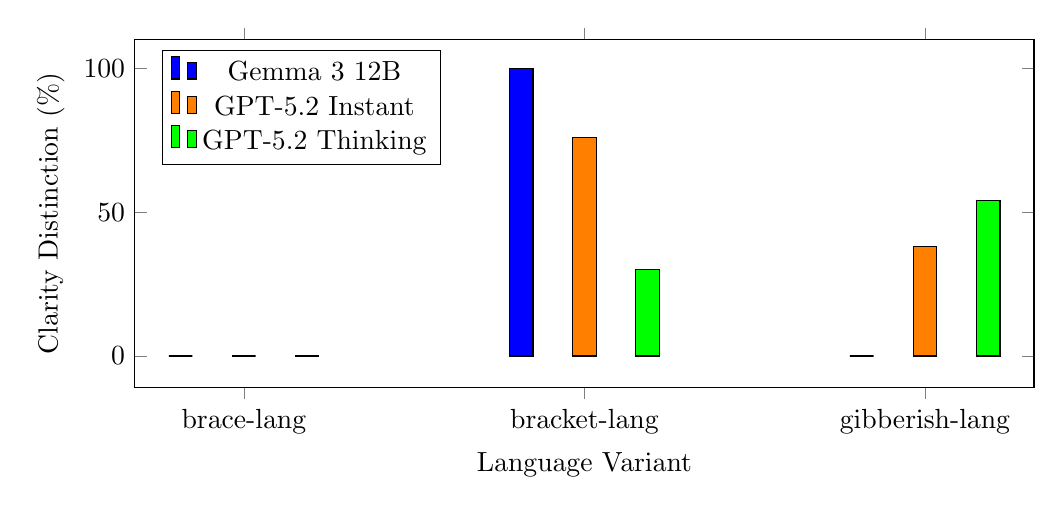
\begin{tikzpicture}
\begin{axis}[
  xlabel={Language Variant},
  ylabel={Clarity Distinction (\%)},
  ymax=110,
  width=13cm,
  height=6cm,
  xtick={1,2,3},
  xticklabels={brace-lang, bracket-lang, gibberish-lang},
  ybar,
  bar width=0.3cm,
  legend pos=north west,
]
\addplot[fill=blue] coordinates {(0.9,0) (1.9,100) (2.9,0)};
\addplot[fill=orange] coordinates {(1.0,0) (2.0,76) (3.0,38)};
\addplot[fill=green] coordinates {(1.1,0) (2.1,30) (3.1,54)};
\legend{Gemma 3 12B, GPT-5.2 Instant, GPT-5.2 Thinking}
\end{axis}
\end{tikzpicture}

\caption{Summary of the experiment results. The height of each bar
indicates the difference in correct fixes between informative
and uninformative error messages relative to the total number of trials
for each language variant, showing Gemma 3 12B and GPT-5.2 Instant models only,
which were able to distinguish the clarity of error messages.}
\label{fig:results-summary}
\end{figure}

%% %% Qualitative explanations for why it is easier for
%% %% top-down parsers to produce clearer error messages include
%% %% \begin{itemize}
%% %%     \item earlier detection of errors due to predictive nature of top-down parsers where unexpected next input token immediately raises an error, in contrast to bottom-up parsers that may need a lot more input to decide whether parsing could continue or not,
%% %%     \item easier to associate the error with the relevant grammar rule in top-down parsers, in contrast to table-driven bottom-up parsers where the error may arise from a combination of multiple reductions and shifts internal parsing states.
%% %% \end{itemize}

%% \begin{figure}[h]
%% \begin{minted}{text}
%% prog    ::= { stmt }
%% stmt    ::= expr ';'
          %% | 'var' ID ';'
          %% | 'fun' ID '(' [params] ')' '{' { stmt } '}'
          %% | 'if' expr 'then' stmt 'else' stmt
          %% | '{' { stmt } '}'
%% params  ::= ID { ',' ID }
%% args    ::= expr { ',' expr }
%% expr    ::= term { '+' term }
%% term    ::= factor { '*' factor }
%% factor  ::= ID | NUM | '(' expr ')' | ID '(' [args] ')'
%% \end{minted}
%% \caption{The grammar (EBNF) for our example language.}
%% \label{fig:core-grammar}
%% \end{figure}



%% \section{Main Body}
%% Write the main body here.

%% \subsection{Code Example}

%% This is an example of code highlighting using the minted package:
%% \begin{minted}{python}
%% def hello_world():
    %% print("Hello, world!")

%% if __name__ == "__main__":
    %% hello_world()
%% \end{minted}

\section{Conclusion}

Write the conclusion here.

\bibliographystyle{plain}
\bibliography{references}

\end{document}
